\documentclass[11pt,a4paper]{article}
\usepackage[utf8]{vietnam}
\usepackage{amsmath,amssymb}
\usepackage{tabularx}
\usepackage{tikz}
\usepackage{xcolor}
\usepackage{fancyhdr}
\usepackage[top=1.8cm, bottom=2.0cm, left=1.8cm, right=1.8cm]{geometry}

\setlength{\parskip}{3pt}
\setlength{\parindent}{0pt}

\pagestyle{fancy}
\fancyhf{}
\renewcommand{\headrulewidth}{0.4pt}
\lhead{\footnotesize \textbf{CHÙA HƯƠNG SƠN -- ÔN THI VÀO 10}}
\rhead{\footnotesize \textbf{ĐỀ THI THỬ CUỐI HỌC KỲ I (ĐỀ SỐ 01)}}
\cfoot{\thepage}

\begin{document}

\noindent
\begin{tabular*}{\linewidth}{@{\extracolsep{\fill}}cc@{}}
\textbf{SỞ GIÁO DỤC VÀ ĐÀO TẠO} & \textbf{ĐỀ KIỂM TRA CUỐI HỌC KỲ I} \\
\textbf{CHÙA HƯƠNG SƠN} & \textbf{NĂM HỌC 2026 -- 2027} \\
\textbf{ĐỀ THI THỬ SỐ 01} & \textbf{MÔN: TOÁN -- LỚP 9} \\
\textit{(Đề thi gồm 03 trang)} & \textit{Thời gian làm bài: 90 phút (không kể thời gian phát đề)} \\
\end{tabular*}

\vspace{2mm}
\noindent
\rule{\linewidth}{0.8pt}

\vspace{1mm}
\noindent
Họ và tên thí sinh: \dotfill Số báo danh: \dotfill

\vspace{2mm}
\noindent
\textbf{\large I. TRẮC NGHIỆM KHÁCH QUAN (7,0 điểm)}

\vspace{1mm}
\noindent
\textbf{Phần 1. Trắc nghiệm nhiều lựa chọn (3,0 điểm).} \textit{Từ câu 1 đến câu 12, thí sinh chọn đáp án đúng nhất trong 4 đáp án A, B, C, D rồi ghi vào bài làm.}

\vspace{1.5mm}
\textbf{Câu 1.} Giá trị của biểu thức $3\sqrt{8} - \sqrt{50} + \sqrt{2}$ bằng\\
\begin{tabularx}{\linewidth}{XXXX}
\textbf{A.} $2\sqrt{2}$. & \textbf{B.} $-2\sqrt{2}$. & \textbf{C.} $4\sqrt{2}$. & \textbf{D.} $0$.
\end{tabularx}

\vspace{1.5mm}
\textbf{Câu 2.} Cho tam giác $MNP$ vuông tại $M$, góc nhọn $\widehat{P} = \beta$. Khẳng định nào sau đây là đúng?\\
\begin{tabularx}{\linewidth}{XXXX}
\textbf{A.} $\sin \beta = \dfrac{MN}{NP}$. & \textbf{B.} $\cos \beta = \dfrac{MN}{NP}$. & \textbf{C.} $\tan \beta = \dfrac{MP}{MN}$. & \textbf{D.} $\cot \beta = \dfrac{MN}{MP}$.
\end{tabularx}

\vspace{1.5mm}
\textbf{Câu 3.} Bất phương trình nào sau đây là bất phương trình bậc nhất một ẩn?\\
\begin{tabularx}{\linewidth}{XXXX}
\textbf{A.} $2x^2 - 3 > 0$. & \textbf{B.} $0x + 5 \le 0$. & \textbf{C.} $-4x + 7 < 0$. & \textbf{D.} $\dfrac{2}{x} - 1 \ge 0$.
\end{tabularx}

\vspace{1.5mm}
\textbf{Câu 4.} Nếu $a < b$ thì bất đẳng thức nào sau đây luôn đúng?\\
\begin{tabularx}{\linewidth}{XXXX}
\textbf{A.} $-3a < -3b$. & \textbf{B.} $2a + 1 < 2b + 1$. & \textbf{C.} $a - 5 > b - 5$. & \textbf{D.} $-a + 2 < -b + 2$.
\end{tabularx}

\vspace{1.5mm}
\textbf{Câu 5.} Căn bậc hai số học của số 81 là\\
\begin{tabularx}{\linewidth}{XXXX}
\textbf{A.} $9$ và $-9$. & \textbf{B.} $9$. & \textbf{C.} $-9$. & \textbf{D.} $81$.
\end{tabularx}

\vspace{1.5mm}
\textbf{Câu 6.} Điều kiện xác định của căn thức $\sqrt{6 - 2x}$ là\\
\begin{tabularx}{\linewidth}{XXXX}
\textbf{A.} $x \ge 3$. & \textbf{B.} $x > 3$. & \textbf{C.} $x \le 3$. & \textbf{D.} $x < 3$.
\end{tabularx}

\vspace{1.5mm}
\textbf{Câu 7.} Với mọi số thực $x \ge 5$, giá trị của biểu thức $\sqrt{(x-5)^2}$ bằng\\
\begin{tabularx}{\linewidth}{XXXX}
\textbf{A.} $x - 5$. & \textbf{B.} $5 - x$. & \textbf{C.} $-(x-5)$. & \textbf{D.} $(x-5)^2$.
\end{tabularx}

\vspace{1.5mm}
\textbf{Câu 8.} Giá trị của $\sqrt[3]{-125}$ bằng\\
\begin{tabularx}{\linewidth}{XXXX}
\textbf{A.} $5$. & \textbf{B.} $-5$. & \textbf{C.} $25$. & \textbf{D.} $-25$.
\end{tabularx}

\vspace{1.5mm}
\textbf{Câu 9.} Trong đường tròn $(O; R)$, công thức tính diện tích hình quạt tròn ứng với cung có số đo $n^\circ$ là\\
\begin{tabularx}{\linewidth}{XXXX}
\textbf{A.} $\dfrac{\pi R^2 n}{360}$. & \textbf{B.} $\dfrac{\pi R n}{180}$. & \textbf{C.} $\dfrac{\pi R^2 n}{180}$. & \textbf{D.} $\dfrac{\pi R n}{360}$.
\end{tabularx}

\vspace{1.5mm}
\textbf{Câu 10.} Cho đường tròn $(O; 5\text{ cm})$ và đường thẳng $d$. Biết khoảng cách từ $O$ đến $d$ là $7\text{ cm}$. Vị trí tương đối của đường thẳng $d$ và đường tròn $(O)$ là\\
\begin{tabularx}{\linewidth}{XXXX}
\textbf{A.} Cắt nhau. & \textbf{B.} Không giao nhau. & \textbf{C.} Tiếp xúc nhau. & \textbf{D.} Trùng nhau.
\end{tabularx}

\vspace{1.5mm}
\textbf{Câu 11.} Cho hai đường tròn $(O; 8\text{ cm})$ và $(O'; 3\text{ cm})$. Biết khoảng cách giữa hai tâm $OO' = 5\text{ cm}$. Vị trí tương đối của hai đường tròn $(O)$ và $(O')$ là\\
\begin{tabularx}{\linewidth}{XXXX}
\textbf{A.} Cắt nhau. & \textbf{B.} Tiếp xúc ngoài. & \textbf{C.} Tiếp xúc trong. & \textbf{D.} Không giao nhau.
\end{tabularx}

\vspace{1.5mm}
\textbf{Câu 12.} Trên đường tròn $(O)$, cho góc ở tâm $\widehat{AOB} = 80^\circ$. Số đo của cung nhỏ $AB$ bằng\\
\begin{tabularx}{\linewidth}{XXXX}
\textbf{A.} $40^\circ$. & \textbf{B.} $160^\circ$. & \textbf{C.} $80^\circ$. & \textbf{D.} $100^\circ$.
\end{tabularx}

\vspace{3mm}
\noindent
\textbf{Phần 2. Trắc nghiệm Đúng -- Sai (2,0 điểm).} \textit{Trong mỗi ý a), b), c), d) ở câu 13 và câu 14, thí sinh chọn đúng hoặc sai và ghi chữ ``Đ'' hoặc ``S'' vào bài làm.}

\vspace{1.5mm}
\textbf{Câu 13.} Xét bài toán thực tế: ``Hai xưởng may được giao kế hoạch may tổng cộng $700$ bộ quần áo bảo hộ y tế. Nhờ cải tiến kỹ thuật, xưởng 1 đã vượt mức $15\%$, xưởng 2 vượt mức $20\%$ so với kế hoạch, do đó cả hai xưởng đã may được tổng cộng $820$ bộ quần áo. Gọi số bộ quần áo xưởng 1 và xưởng 2 phải may theo kế hoạch lần lượt là $x$ và $y$ ($x, y \in \mathbb{N}^*, x, y < 700$).''\\
Xét tính đúng sai của các khẳng định sau:
\begin{center}
\begin{tabularx}{\linewidth}{|X|c|c|}
\hline
\textbf{Khẳng định} & \textbf{Đúng} & \textbf{Sai} \\
\hline
a) Theo kế hoạch, hai xưởng may $700$ bộ nên ta có phương trình: $x + y = 700$. & & \\
\hline
b) Số bộ quần áo xưởng 1 và xưởng 2 làm được trong thực tế lần lượt là $1{,}15x$ và $1{,}2y$. & & \\
\hline
c) Hệ phương trình biểu thị mối quan hệ giữa $x$ và $y$ là: $\begin{cases} x + y = 700 \\ 1{,}15x + 1{,}2y = 800 \end{cases}$. & & \\
\hline
d) Theo kế hoạch, xưởng 1 phải may $400$ bộ và xưởng 2 phải may $300$ bộ quần áo. & & \\
\hline
\end{tabularx}
\end{center}

\vspace{2mm}
\textbf{Câu 14.} Cho đường tròn $(O; 5\text{ cm})$ và điểm $M$ nằm ngoài đường tròn sao cho $OM = 13\text{ cm}$. Từ $M$ kẻ hai tiếp tuyến $MA, MB$ với $(O)$ ($A, B$ là các tiếp điểm). Gọi $H$ là giao điểm của $OM$ và $AB$.\\
Xét tính đúng sai của các khẳng định sau:
\begin{center}
\begin{tabularx}{\linewidth}{|X|c|c|}
\hline
\textbf{Khẳng định} & \textbf{Đúng} & \textbf{Sai} \\
\hline
a) Tam giác $MAO$ vuông tại $A$ và có độ dài đoạn thẳng $MA = 12\text{ cm}$. & & \\
\hline
b) Đoạn thẳng $OM$ vuông góc với dây cung $AB$ tại $H$. & & \\
\hline
c) Chu vi của hình tròn $(O)$ bằng $25\pi\text{ cm}$. & & \\
\hline
d) Độ dài dây cung $AB$ bằng $\dfrac{120}{13}\text{ cm}$. & & \\
\hline
\end{tabularx}
\end{center}

\vspace{3mm}
\noindent
\textbf{Phần 3. Trắc nghiệm trả lời ngắn (2,0 điểm).} \textit{Từ câu 15 đến câu 18, thí sinh chỉ ghi kết quả cuối cùng vào bài làm.}

\vspace{1.5mm}
\textbf{Câu 15.} Nghiệm của bất phương trình $3(x + 2) - 5 > 2(2x - 1) + 1$ là $\dots\dots\dots$

\vspace{1.5mm}
\textbf{Câu 16.} Giá trị của biểu thức $N = \sqrt{(\sqrt{7} - 3)^2} + \sqrt{7}$ bằng $\dots\dots\dots$

\vspace{1.5mm}
\noindent
\begin{minipage}[c]{0.65\linewidth}
\textbf{Câu 17.} Một tòa tháp có bóng trên mặt đất dài $15\text{ m}$. Biết rằng góc tạo bởi tia nắng mặt trời với mặt đất tại thời điểm đo là $55^\circ$ (xem hình vẽ bên). Tính chiều cao của tòa tháp (làm tròn kết quả đến chữ số thập phân thứ hai của mét).
\end{minipage}\hfill
\begin{minipage}[c]{0.32\linewidth}
\centering
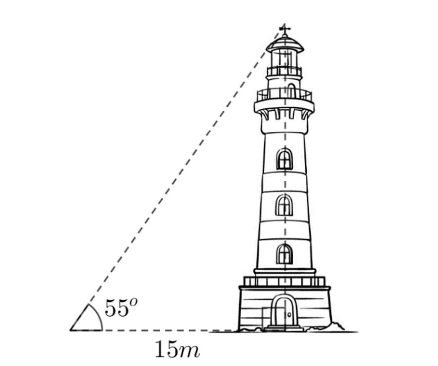
\includegraphics[width=3.6cm]{hinh_cau_17.png}
\end{minipage}

\vspace{1.5mm}
\textbf{Câu 18.} Một chiếc quạt giấy xòe ra tạo thành một hình quạt tròn có bán kính $R = 20\text{ cm}$ và góc ở tâm tương ứng là $120^\circ$. Tính diện tích phần giấy làm bề mặt quạt (lấy $\pi \approx 3{,}14$, làm tròn kết quả đến chữ số thập phân thứ nhất, đơn vị: $\text{cm}^2$).

\vspace{4mm}
\noindent
\textbf{\large II. TỰ LUẬN (3,0 điểm).} \textit{Thí sinh trình bày lời giải chi tiết vào tờ giấy thi.}

\vspace{2mm}
\textbf{Câu 19 (1,0 điểm).}
\begin{itemize}
  \item[a)] \textit{(0,5 điểm)} Giải hệ phương trình: $\begin{cases} 3x - y = 7 \\ 2x + 3y = 1 \end{cases}$.
  \item[b)] \textit{(0,5 điểm)} Cho biểu thức $A = \left( \dfrac{\sqrt{x}}{\sqrt{x} + 3} + \dfrac{2\sqrt{x}}{\sqrt{x} - 3} - \dfrac{3x + 9}{x - 9} \right) : \dfrac{\sqrt{x} - 1}{\sqrt{x} - 3}$ với $x > 0, x \ne 9, x \ne 1$. Rút gọn biểu thức $A$.
\end{itemize}

\vspace{2mm}
\textbf{Câu 20 (1,5 điểm).} Cho đường tròn $(O; R)$, đường kính $AB$. Trên tiếp tuyến của đường tròn $(O)$ tại $A$, lấy điểm $M$ ($M$ khác $A$). Từ $M$ vẽ tiếp tuyến thứ hai $MC$ với đường tròn $(O)$ ($C$ là tiếp điểm).
\begin{itemize}
  \item[a)] \textit{(0,75 điểm)} Chứng minh rằng bốn điểm $A, M, C, O$ cùng nằm trên một đường tròn.
  \item[b)] \textit{(0,75 điểm)} Kẻ $CH$ vuông góc với $AB$ tại $H$ ($H \in AB$). Đoạn thẳng $MB$ cắt $(O)$ tại điểm thứ hai là $K$ và cắt $CH$ tại $N$. Chứng minh rằng: $MA^2 = MK \cdot MB$ và $N$ là trung điểm của đoạn thẳng $CH$.
\end{itemize}

\vspace{2mm}
\textbf{Câu 21 (0,5 điểm).}
\begin{itemize}
  \item[a)] \textit{(0,25 điểm)} Một hộ gia đình muốn xây dựng một bể chứa nước sinh hoạt ngầm không có nắp đậy dạng hình hộp chữ nhật với đáy là hình vuông, có thể tích là $32\text{ m}^3$. Hãy tìm các kích thước của bể (chiều dài, chiều rộng đáy và chiều sâu) để diện tích vật liệu xây dựng (gồm đáy và 4 mặt xung quanh) là nhỏ nhất.
  \item[b)] \textit{(0,25 điểm)} Cho ba số thực dương $x, y, z$ thỏa mãn điều kiện $x + y + z \le 3$. Tìm giá trị nhỏ nhất của biểu thức:
  \[
  P = x^2 + y^2 + z^2 + \dfrac{2}{x} + \dfrac{2}{y} + \dfrac{2}{z}.
  \]
\end{itemize}

\vspace{4mm}
\begin{center}
\textbf{---------- HẾT ----------}\\
\textit{(Cán bộ coi thi không giải thích gì thêm)}
\end{center}

\end{document}
